\documentclass[12pt, fleqn, titlepage]{article}

\usepackage[utf8]{inputenc}
\usepackage[T2A]{fontenc}
\usepackage{amssymb,amsmath,mathrsfs,amsthm}
\usepackage[russian]{babel}
\usepackage[pdftex]{graphicx}

\usepackage[footnotesize]{caption}
\usepackage{indentfirst}
\usepackage{mathtools}

\textheight=24cm
\textwidth=16cm
\oddsidemargin=5mm
\evensidemargin=-5mm
\marginparwidth=36pt
\topmargin=-1.5cm
\footnotesep=3ex
\raggedbottom
\tolerance 3000
\clubpenalty=10000
\widowpenalty=10000
\renewcommand{\baselinestretch}{1.1}
\renewcommand{\baselinestretch}{1.5} 

\newtheorem{Def}{Определение}

\usepackage{pgfplots}
\pgfplotsset{compat=1.16}

\begin{document}

    \begin{titlepage}
        \begin{center}
            Московский государственный университет имени М. В. Ломоносова
            
            
\includegraphics[width=50mm]{./pics/msu.jpg}
            
            \bigbreak
            Факультет Вычислительной Математики и Кибернетики

            Кафедра Математических Методов Прогнозирования

            \vspace{10mm}

            \textbf{\large КУРСОВАЯ РАБОТА}

            \vspace{10mm}

            \textbf{\Large <<Анализ структуры вершин транспортных сетей>>}

            \vspace{10mm}

            \textbf{\Large <<Analysis of Vertex Structure in Transport Networks>>}

            \vspace{10mm}
            
            \begin{flushright}
                \parbox{0.5\textwidth}{
                    Выполнил:

                    студент 317 группы
                    
                    Сидоров Леонид Станиславович

                    \vspace{5mm}

                    Научный руководитель:

                    к.ф.-м.н.
                    
                    Майсурадзе Арчил Ивериевич
                }
            \end{flushright}
            \vspace{\fill}
            Москва, 2021   
        \end{center}
    \end{titlepage}

    \newpage
    \begin{center}
        \textbf{Аннотация}
    \end{center}

    Развитие телекоммуникационных технологий и проникновение смартфонов в нашу жизнь привели к тому, 
    то по перемещениям мобильных устройств можно достаточно точно измерять транспортные потоки. Поэтому 
    проблема предсказания трафика в наше время уже не так актуальна, а данные о потоках используются 
    в качестве метрики, отражающей определённые процессы в городе. 

    Так, информация о поездках между станциями метро может характеризовать шаблоны использования 
    соответствующих станций и прилегающих к ним территорий, которые могут оказаться спальными районами, 
    точками интереса, пересадочными узлами или чем-то ещё. Любые изменения в таких шаблонах являтюся отражением 
    некоторых процессов в городе, иногда требующих незамедлительной реакции. В данном докладе будут рассмотрены 
    существующие и предложены новые способы поиска таких паттернов. 
    \newpage

    \newpage
        \tableofcontents
    \newpage

    \section{Введение}

    Современные мегаполисы, особенно такие как Москва, представляют собой невероятные структуры, функционирование которых 
    день ото дня поддерживается огромным количеством подсистем, отвечающих за каждодневные нужды граждан. Одной из таких 
    структур является транспортная сеть. В этой работе мы изучим поведение значительного её подмножества, известного как 
    метрополитен.

    Но прежде обратим внимание на основные классы задач, с которыми сталкиваются специалисты по транспорту во время своей 
    работы.

    Традиционно, исследование транспорта предполагало какой-то прогноз, будь то поток пассажиров, направление движения или 
    что-либо ещё. Однако, даже абстрагируясь от прогнозируемой величины, мы получаем огромное количество задач, различающихся 
    типом входных данных. Например, источником данных может служить транспортная карта \cite{namiot2017survey}, 
    которая фиксирует факт начала поездки, или карта, считывающая информацию и о начале, и о конце каждого путешествия 
    \cite{duan2018understanding}. В первом случае нам приходится полагаться на различные эвристики, например, анализ 
    точки старта следующей поездки.

    Однако данные, как в нашем случае, могут собираться и другим образом. Здесь нам на помощь приходят телекоммуникационные 
    операторы, которые обеспечивают наличие связи в метро. Как известно, с некоторыми ограничениями \cite{niu2015novel}, 
    мобильные операторы способны отслеживать перемещение почти любого мобильного девайса, то есть узнавать маршрута пассажиров. 
    В этом случае фактом входа в метро является переключение телефона с наземной базовой станции на подземную, а выход, соответственно,~--- 
    с подземной на надземную, то есть оператор знает начальную и конечную точку любой поездки. Далее эти данные агрегируются по 
    времени с целью защиты персональных данных \cite{sweeney2002k} и записываются в виде матрицы корреспонденций \cite{necr2019}.

    В таких матрицах показывается количество перемещений между двумя пунктами, представленными в строках и столбцах матрицы. 
    Эти перемещения относятся, вообще говоря, произвольному фиксированному временному интервалу (одному для каждого элемента 
    матрицы). То есть в матрице корреспонденций $M$, элемент $m_{ij}$ показывает количество
    перемещений за заданный временной интервал $t$ от пункта $i$ до пункта $j$.

    Матрица корреспонденций может быть как конечной целью анализа \cite{djukic2012efficient}, так и исходными данными 
    для какой-либо другой задачи прогнозирования.
    
    Потоки пассажиров в транспортной сети могут изменяться под давлением внешних факторов. Будь то открытие нового автобусного 
    маршрута или возникновение крупного пересадочного узла, эти события не могут описаны в матрице корреспонденций. Однако 
    подобные транспортные события непосредственно влияют на саму матрицу корреспонденций, поэтому она может выступать в роли 
    индикатора этих событий или служить универсальной мерой воздействия подобных ситуаций на транспортную систему \cite{namiot2020}.

    Подобная информация, полученная посредством анализа матрицы корреспонденций, сама может служить исходной информацией 
    для прогнозирования транспортных потоков. Например, оптимизация движения поездов на каком-либо маршруте 
    метрополитена, очевидно, требует наличия данных о пассажиропотоке на станциях этого маршрута.
    
    Матрицы корреспонденции для метро (железной дороги) проще для обработки, поскольку здесь, по очевидным причинам, 
    маршруты фиксированы, происходящее при самом перемещении мы не рассматриваем, и в используемых моделях есть только 
    один тип выделенных объектов – станции.

    В данной работе будут рассмотрены новые методы выявления транспортных ситуаций на основе матрицы корреспонденций, построенной 
    с помощью данных о поездках пассажиров московского метрополитена за февраль 2018 года. Эти данные были собраны с помощью 
    мобильных операторов связи описанным выше способом. Также они использовались в \cite{namiot2020, necr2019}, 
    однако там рассматривалась задача предсказания будущего трафика. Проблема, решаемая мной, уже ставилась в \cite{namiot2021}, 
    но пока не получила решения.

    \section{Обзор литературы}

    Как уже упоминалось ранее, задача выявления транспортных ситуаций является относительно новой в сфере анализа трафика. 
    Тем не менее, в контексте решения других задач исследователи прибегали к методам преобразования матрицы корреспонденций к 
    другому признаковому представлению и качественному анализу её данных. Рассмотрим несколько релевантных примеров.

    \begin{figure}
        \centering
        \captionsetup{justification=centering}
        \begin{minipage}{.5\textwidth}
          \centering
          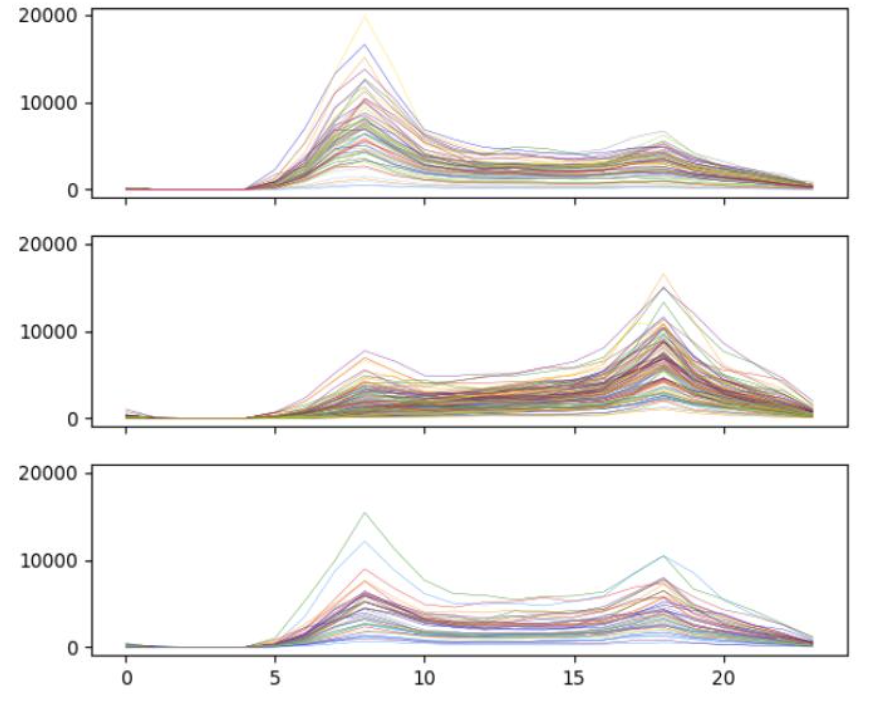
\includegraphics[width=\linewidth]{pics/art1_dist.png}
          \captionof{figure}{Разбиение станций по \\соотношению пиков \cite{necr2019}.}
          \label{art1_dist}
        \end{minipage}%
        \begin{minipage}{.5\textwidth}
          \centering
          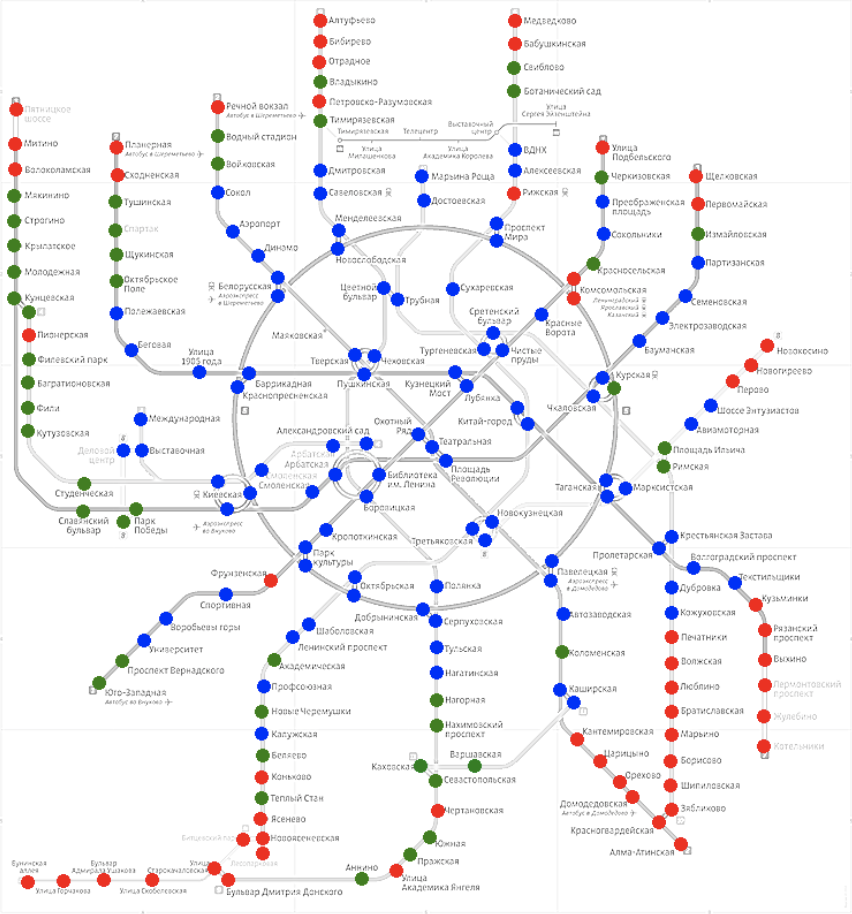
\includegraphics[width=.75\linewidth]{pics/art1_map.png}
          \captionof{figure}{Зонирование города по \\величине пиков \cite{necr2019}.}
          \label{art1_map}
        \end{minipage}
        \end{figure}

    В работе \cite{necr2019} производится предсказание трафика на основе матрицы корреспонденций. Предсказание производится  с 
    помощью таких классических алгоритмов машинного обучения, как метод K ближайших соседей, линейная регрессия и многослойная 
    нейронная сеть. Однако, мы не можем подать матрицу корреспонденций в изначальном виде на вход этим алгоритмам, сначала её 
    надо преобразовать в таблицу с признаковыми описаниями объектов, а именно пар станций с заданным направлением движения.

    Рассмотрим интенсивность притока пассажиров на каждую станцию в течение каждого часа суток. По распределению нагрузки 
    станции можно разбить на три большие категории: рабочая зона города, жилищная зона и зона смешанного типа (Рис. \ref{art1_dist}). 
    Для распределения станций по этим группам авторы используют довольно простой критерий. У станций из рабочей зоны пик 
    транспортной активности (прибывает максимум пассажиров) приходится на утро, а у станций из жилищной зоны на вечер. 
    У станций же смешанного типа ни утренний, ни вечерний пик не преобладает над другим.

    Пик в подобном представлении считается преобладающим, если он превосходит второй пик более чем в $1.5$ раза. Результат 
    зонирования представлен на Рис. \ref{art1_map}, синий цвет соответствует рабочей зоне, красный жилищной, а зелёный 
    смешанной. Как мы видим, подобная карта имеет определённую структуру и укладывается в 
    базовые представления об устройстве города: спальные районы находятся на периферии, а рабочие в центре.

    Кроме того, авторы эмпирически подтвердили гипотезу о том, что пассажиропотоки на соседних станциях метрополитена 
    коррелирует друг с другом и тоже использовали эту информацию для анализа. Также учитывая исторические данные 
    пассажиропотока, они использовали метод главных компонент для получения итогового признакового описания.

    Ещё одним примером анализа транспортных ситуаций является работа \cite{duan2018understanding}, в которой изучались 
    транспортные системы двух городов Китая: Шанхая и Шеньчженя. Здесь основным инструментом является сингулярное 
    разложение (Singular value decomposition, SVD).

    \begin{figure}[ht]
        \centering
        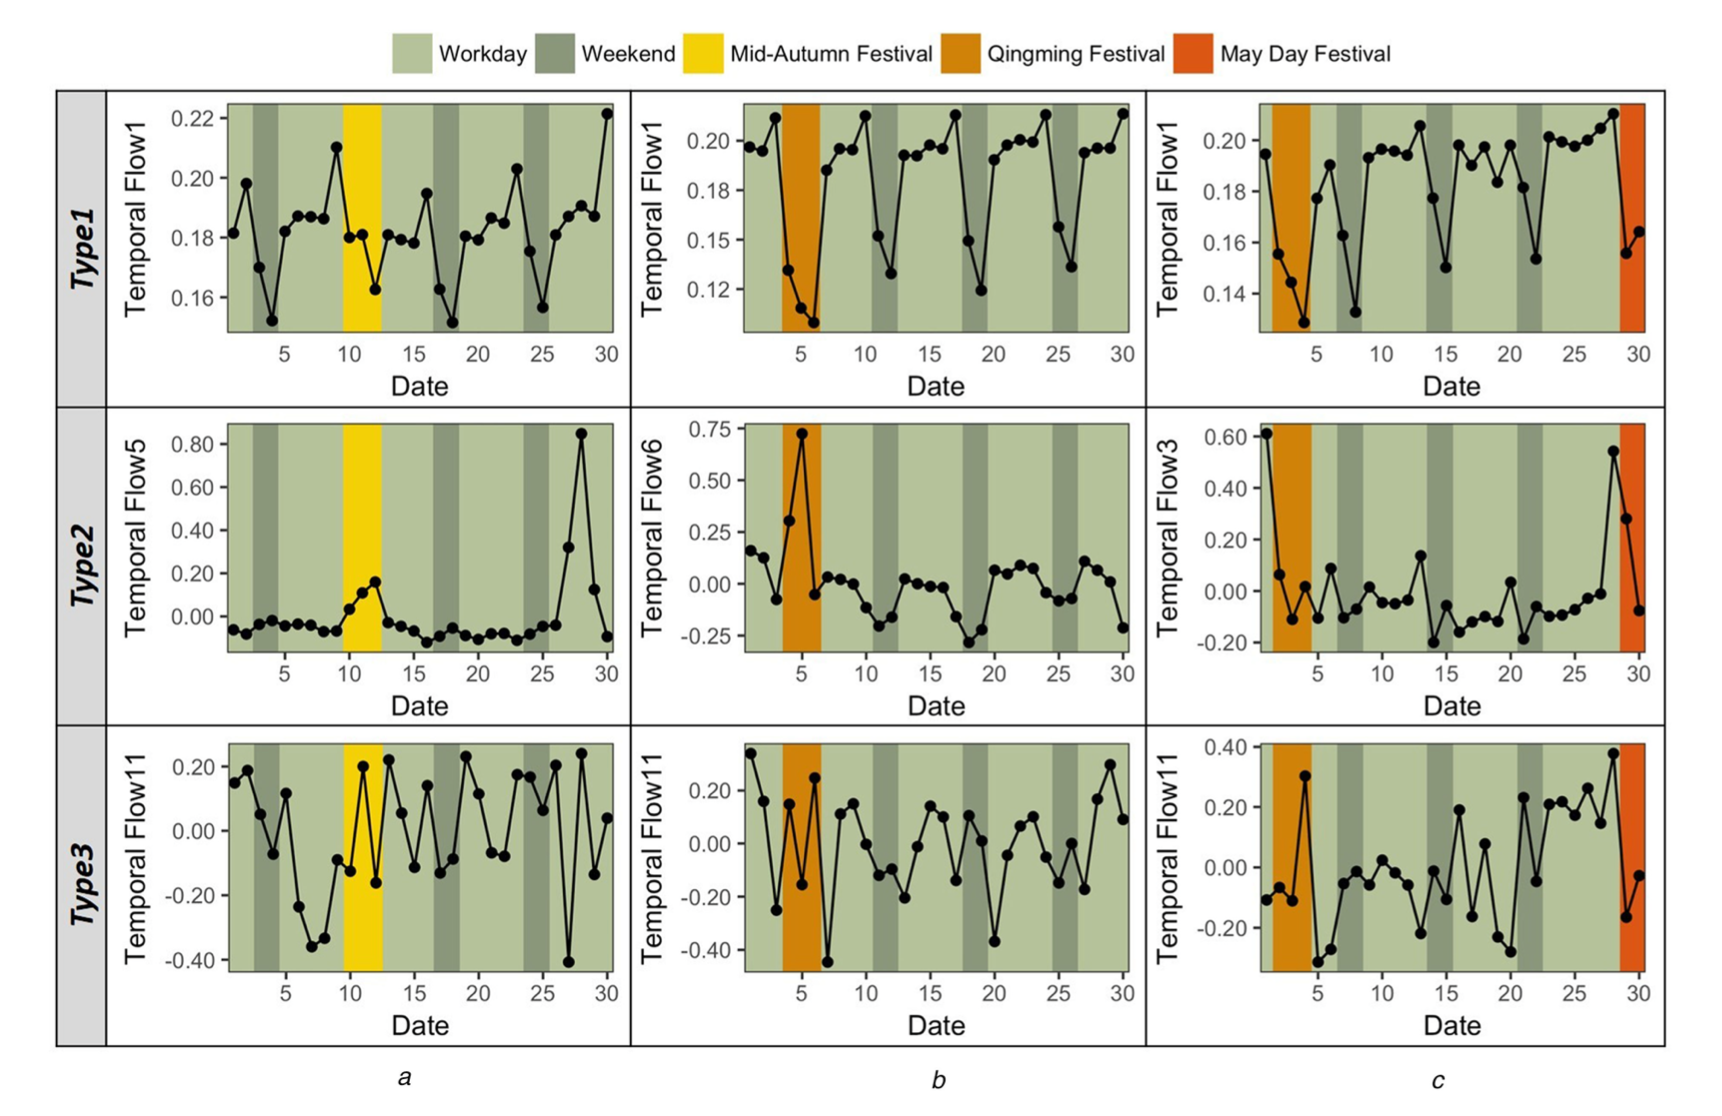
\includegraphics[scale=0.5]{pics/flows.png}
        \caption{Примеры временных потоков \cite{duan2018understanding}.}
        \label{flows}
    \end{figure}

    Исходная матрица корреспонденций $M$ была разложена при помощи SVD:

    $$
    M = USV^T = \sum_{i = 1}^r \delta_i u_i v^T_i,
    $$

    где $S$~--- матрица сингулярных чисел, $U$~--- матрица временных потоков (\textit{temporal flow}), а $V$~--- 
    матрица характера спроса (\textit{demand pattern}). 

    Как можно было понять из названия, в случае разложения матрицы корреспонденций полученные матрицы имеют смысл 
    в контексте решаемой задачи. А именно строки $U$ называются временными потоками и отражают характер пассажиропотока 
    всей транспортной системы за рассматриваемый период, столбцы $V$ называются векторами характера спроса и являются базисом для 
    разложения пассажиропотока, а на диагонали $S$, как обычно, находятся сингулярные числа, отражающие вклад 
    каждого элемента в разложение.

    Также дальнейшие исследования показали, что при отбрасывании всех пар векторов $(u_i, v_i)$, кроме трёх, соответствующих 
    максимальным сингулярным числам, полученная матрица $\hat{M} = \sum_{i = 1}^3 \delta_i u_i v^T_i$ будет отличаться от исходной 
    матрицы $M$ менее, чем на $10\%$. То есть три временных потока характеризуют большую часть пассажиропотока всей системы. 

    Авторы статьи не останавливаются на этом и приводят классификацию этих трёх основных потоков. Как мы видим на Рис. \ref{flows}, 
    потоки первого типа отражают недельные паттерны перемещения, люди ездят по-разному в выходные и рабочие дни; потоки второго типа 
    отвечают за неординарные всплески активности, например, праздники или, как в случае столбца \textit{a}, закрытие некоторых 
    станций и перераспределение пассажиропотока; в потоках же третьего типа каких-либо закономерностей обнаружено не было, они являются 
    шумовой составляющей. Изначально мы не знаем типы потоков, однако их довольно легко установить по названным выше критериям. 
    
    Таким образом, на основе матрицы корреспонденций мы можем анализировать паттерны движения пассажиров и своевременно выявлять 
    реакцию транспортной системы на те или иные внешние события.

    \section{Постановка задачи}

    \subsection{Природа данных}

    Рассматриваем движение людей между станциями метро. Исходные объекты - это отдельные поездки людей. 
    Для каждой поездки известны станция и время отправления, станция и время прибытия. Нам же эти данные 
    поступили в агрегированном виде, объектом считается пара станций и некоторый получасовой интервал. 
    Следовательно, мы можем представить их в виде матрицы корреспонденций, хотя и с некоторыми оговорками. 
    Дело в том, что поездки в московском метрополитене могут занимать больше чем полчаса, то есть сумма 
    элементов матрицы корреспонденций на каждом временном срезе не является постоянной.

    Как уже говорилось, данные собирались при помощи сим карт в телефонах пассажиров. Сотовые станции размечались на 
    “наземные” и “подземные”. Регистрировались переключения телефонов пассажиров между этими двумя видами станциями. 
    Переход от “наземной” к “подземной” означал “вход в метро”, а наоборот~--- “выход из метро”. 

    Очевидно, при таком подходе неизбежны некоторые погрешности измерения. 
    Данные от операторов мобильной связи подвергаются укрупнению как по времени, так и по местоположению, также 
    с целью дополнительной анонимизации эти данные собираются с использованием алгоритмов \textit{temporal cloaking} и 
    \textit{spatial cloaking}, скрывающих точное местоположение пользователя \cite{niu2015novel}.

    На Рис. \ref{disappearance} изображены абсолютное и относительное количества людей, “пропадающих” в московском 
    метрополитене за каждый день рассматриваемого периода, они заходят в метро, но не выходят обратно. 

    \begin{figure}[ht]
        \centering
        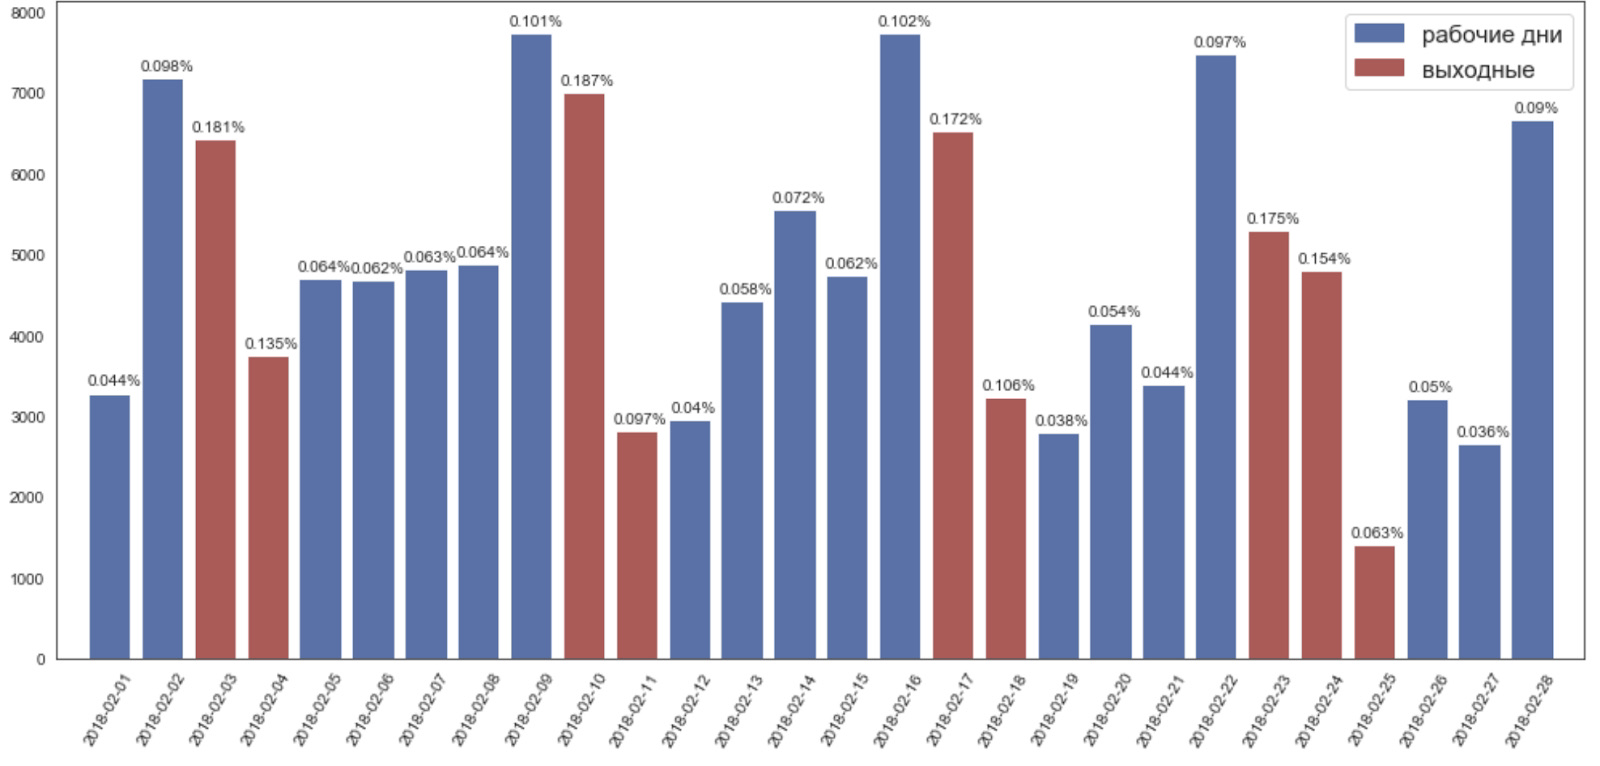
\includegraphics[scale=0.25]{pics/disappearance.png}
        \caption{Разница между количеством зашедших и вышедших из метро пассажиров.}
        \label{disappearance}
    \end{figure}

    Ясно, что таким образом нельзя учесть поездки вообще всех пассажиров, ведь кто-то может и не носить с собой 
    телефона вовсе. Но, принимая во внимание современный уклад жизни, можно считать, что количество таких людей пренебрежительно мало. 

    Доступная мне выборка состоит только из поездок, совершённых в феврале 2018 года. Для каждого интервала и 
    каждой пары станций записано, сколько людей в этот получасовой интервал стартовало с первой станции и сколько 
    людей в этот же интервал приехало на вторую. Это могут быть разные люди. 

    \begin{center}
    \begin{tabular}{ |c|c|c|c|c| } 
    
        \hline
        уникальный & станция & станция & число & число \\
        получасовой & отправления & прибытия & выехавших со & прибывших на \\
        интервал &  &  & станции & станцию \\
        (дата и время) &  &  & отправления & прибытия \\
        \hline
        \multicolumn{5}{c}{\footnotesize Таблица 1.
        Формат исходных данных.} \\
    
    \end{tabular}
    \end{center}

    \subsection{Методы анализа}

    Для начала введём формальное определение матрицы корреспонденций.

    \begin{Def}
            Рассмотрим транспортную сеть как планарный граф $G = (V, E)$. С каждой вершиной ассоциируется 
            некоторая станция как место отправления (исток, $O \in V$) или прибытия (сток, $D \in V$) пассажиров. 
            Тогда {\bf матрица корреспонденций} имеет вид 
            $$p(t) = \{p_{ij}(t), i \in O, j \in D, t \in T \}$$, 
            где $[0, T]$~--- рассматриваемый временной интервал.
    \end{Def}

    Отметим, что датой работы метро является не совсем астрономическая дата. 
    Условная смена дат приходится на час ночи. Предполагается, что, когда метро закрыто на ночь, все люди должны его покинуть. 
    Люди могут входить в метро только с момента открытия и должны покинуть его до момента закрытия.

    В ходе исследования было сформулировано две задачи: анализ потоков пассажиров и 
    предсказание времени поездки между произвольной парой станций.

    Потоком мы будем называть пару станций, между которыми люди преимущественно ездят в одном направлении, то 
    есть в течение дня не возвращаются по тому же маршруту. Направление потока~--- станция прибытия 
    большинства пассажиров.

    Первая задача предполагает использование критериев однородности двух статистических выборок и 
    построение с их помощью матрицы потоков между всеми станциями метрополитена. Используя эту матрицу 
    мы можем выделить стоки (истоки), то есть станции, куда направлены (откуда исходят) большинство потоков. 
    Эта информация является весомой характеристикой транспортной системы, так как она выявляет точки притяжения 
    людей и помогает искать транспортные узлы, снабжающие систему большим количеством пассажиров извне.
    
    Вторая задача заключается построении распределения времени поездки 
    между произвольной парой станций. Анализ модальности этого распределения позволил бы нам выявить 
    наличие или отсутствие альтернативных маршрутов, то есть альтернативных путей между парой станций, 
    отличающихся от кратчайшего, но тем не менее популярных среди пассажиров. Такая информация может 
    выявлять какие-либо внештатные ситуации или сигнализировать о недостаточной информированности людей, 
    выбирающих неоптимальный маршрут.

    \section{Анализ потоков пассажиров}

    Для начала рассмотрим две произвольные станции московского метрополитена. В нашем примере это Университет и Речной вокзал. 
    Мы хотим проверить гипотезу о том, что пара этих станций не является потоком, 
    то есть, что для замкнутой системы из Университета и Речного вокзала на каждую станцию приезжает и уезжает равное число людей. 
    Считается, что все дни месяца равноправны, то есть мы не разделяем их 
    на выходные и будние или как-либо ещё.

    \subsection{Подготовка данных}

    Для начала выделим из общей совокупности интересующие нас поездки, а именно поездки от 
    Университета до Речного вокзала и наоборот (это один элемент матрицы корреспонденций $p_{ij}(t)$). 
    Их следует разделить на две отдельные выборки 
    для дальнейшего сравнения~--- поездки в одну и в другую стороны. 
    Станции отправки и прибытия нам при этом уже не нужны, эта информация уже учтена при составлении выборок.

    Теперь проведём укрупнение по датам для каждой выборки, учитывая при этом условную смену 
    дат метрополитена. Для этого вычтем час из каждого показателя даты и времени. 
    После чего избавимся от времени в показателе интервала, полученный столбец является ключом группы. 
    Проведем по нему укрупнение. При этом агрегируем число прибывших и число отправившихся при помощи суммы.

    \begin{center}
    \begin{tabular}{ |c|c|c| } 
    
        \hline
        дата (смена дат — время & число выехавших со & число прибывших на \\
        закрытия метро) & станции отправления & станцию прибытия \\
        \hline
        2018-02-01 & 96 & 96 \\
        2018-02-02 & 108 & 105 \\
        2018-02-03 & 38 & 39 \\
        2018-02-04 & 20 & 21 \\
        2018-02-05 & 105 & 101 \\
        \hline
        \multicolumn{3}{c}{\footnotesize Таблица 2.
        Пример данных, агрегированных для поиска потоков.} \\
    
    \end{tabular}
    \end{center}

    При этом столбцы 2 и 3 содержат результаты измерений одной и той же величины 
    (число выехавших/прибывших пассажиров), потому что пропажа людей при поездке в поезде не предусмотрена. 
    Тем не менее часто значения в этих столбцах немного отличаются друг от друга. 
    Это связано с описанными выше причинами, а именно алгоритмами анонимизации \cite{niu2015novel}.
    Однако эти отклонения составляют не более $5\%$ от числа пассажиров, поэтому для простоты изложения 
    далее в работе, пока не оговорено иного, в качестве экспериментальной выборки будет использоваться только второй столбец.

    \subsection{Постановка статистической задачи}

    В этом разделе мы рассмотрим 2 возможные постановки статистической задачи для исходных данных. 
    Считая количество пассажиров случайной величиной, которую мы не можем предсказать заранее с идеальной точностью, 
    проверим гипотезу однородности для двух случаев: 2 независимые выборки (все даты равноправны) 
    и 2 парные выборки (сопоставление по датам). Но сначала введём определение критерия однородности.

    \begin{Def}
            {\bf Критерий однородности}~--- это критерий проверки гипотезы о том, что две (или более) 
            выборки взяты из одного распределения вероятностей. 

            Они бывают двух типов:
            \begin{itemize}
            \item {\bf Непараметрические (свободные от распределения) критерии 
            однородности} не предполагают присутствия какой-либо фундаментальной информации о законе распределения. 

            \item {\bf Параметрические критерии однородности} используются при наличии каких-либо дополнительных предположений о законе распределения вероятностей.
            \end{itemize}
    \end{Def}


    Пусть $\xi$~--- это число человек, прибывших на Речной вокзал c Университета, а $\eta$~--- наоборот, 
    c Речного вокзала на Университет. По изначальной постановке задачи мы не различаем дни месяца. 
    Следовательно, полученные в предыдущем пункте два набора данных можно 
    рассматривать как выборку, порождённую случайной величиной $\xi$ (её обозначим как $x = (x_1, x_2, \dots , x_n)$), 
    и выборку, порождённую случайной величиной $\eta$ (её обозначим как $y = (y_1, y_2, \dots , y_n)$). 
    Эти выборки имеют одинаковый размер $n = 28$  (число дней в феврале 2018 года).

    В итоге исходная задача сводится к проверке гипотезы однородности выборок $x$ и $y$. 
    Изобразим их гистограммы для представления природы распределений $\xi$ и $\eta$.

    \begin{figure}[ht]
        \centering
        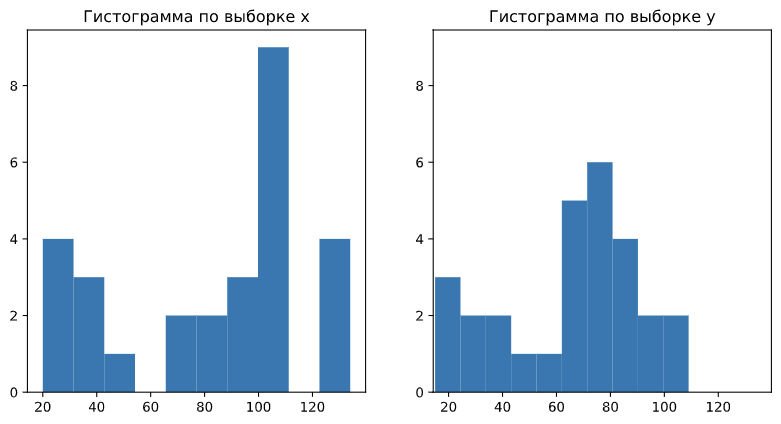
\includegraphics[scale=0.4]{pics/dists.png}
        \caption{Гистограммы выборок $x$ и $y$.}
        \label{dists}
    \end{figure}

    Изучая гистограммы выборок $x$ и $y$ (Рис. \ref{dists}), можно прийти к выводу о том, что распределения $\xi$ и $\eta$ отличны от нормального. 
    Также мы можем применить критерий Шапиро-Уилка для проверки этих выборок на нормальность \cite{shapiro}. 
    Это один из наиболее эффективных критериев проверки нормальности распределения случайных величин \cite{shapiro_power, kobzar2012asm}.
    В качестве альтернативы в нём рассматривается отклонение коэффициентов асимметрии и эксцесса 
    исходного распределения от нормального.
    
    Положим, уровень значимости $\alpha = 10\%$. Применяя критерий Шапиро-Уилка к выборкам $x$ и $y$, 
    я получил значения уровня значимости (\textit{p-value}) $0.006$ и $0.0928$ соответственно, что позволяет нам отвергнуть нулевую гипотезу. 
    Поэтому нам стоит искать непараметрический критерий.

    Теперь рассмотрим 2 противоположных предположения о природе данных.

    \subsubsection{Парные выборки}

    В этом случае мы предполагаем, что выборки парные, 
    то есть каждому $x_i$ соответствует $y_i$ для $i = 1, \dots , n$. В этом случае уместно ввести 
    величину $z_i = x_i - y_i$, $i = 1, \dots , n$ и рассмотреть ранговый критерий Вилкоксона \cite{wilcoxon}, альтернативной 
    гипотезой в котором является ассиметричность распределения, характеризующего выборку $z = (z_1, z_2, \dots , z_n))$. 
    Критерий можно применять при $n > 20$, что удовлетворяет нашим данным.

    \subsubsection{Независимые выборки}

    В этот раз мы считаем выборки $x$ и $y$ независимыми, то есть порядок расположения элементов в 
    каждой из них не имеет значения. Тогда применим критерий Манна-Уитни, который является обобщением 
    рангового критерия Вилкоксона для случая независимых выборок \cite{mannwhitneyu}. Соответственно, альтернативная гипотеза 
    и мощность в нём остаются теми же.
    
    Однако альтернатива в этих критериях не позволяет со всей уверенностью отвергнуть нулевую гипотезу 
    в случае превышения допустимого уровня значимости. Поэтому было решено также рассмотреть двухвыборочный 
    критерий Колмогорова-Смирнова, который оценивает разницу эмпирических функций распределения, а значит, 
    даёт однозначный ответ на наш вопрос \cite{ks_2samp}.

    \subsection{Результаты эксперимента}

    После применения всех вышеперечисленных критериев к рассматриваемым выборкам, мы получили следующие результаты.

    \begin{center}
    \begin{tabular}{ |c|c|c| } 
        
        \hline
        wilcoxon & mannwhitneyu & ks\_2samp \\
        \hline
        0.00024 & 0.00835 & 0.01089 \\
        \hline
        \multicolumn{3}{c}{\footnotesize Таблица 3.
        Значения p-value для различных критериев однородности} \\
        \multicolumn{3}{c}{\footnotesize 
        на паре станций Университет и Речной вокзал.} \\
        
    \end{tabular}
    \end{center}

    Все три постановки задачи позволяют нам вполне уверенно отвергнуть нулевую гипотезу, и сказать, что между 
    Университетом и Речным вокзалом существует поток. В качестве направления потока мы будем выбирать ту станцию, 
    на которую приезжает больше пассажиров. В нашем случае на Университет суммарно приехало \textbf{1830} человек, а 
    на Речной вокзал~--- \textbf{2332}. Следовательно, поток направлен на Речной вокзал.
    \begin{figure}[ht]
        \centering
        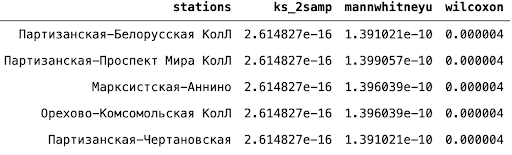
\includegraphics[scale=0.5]{pics/min_ks_2samp.png}
        \caption{Сравнение минимальных значений p-value критерия Колмогорова-Смирнова с результатами других критериев.}
        \label{min_ks_2samp}
    \end{figure}

    Хоть критерии Вилкоксона и Манна-Уитни и дают меньшее значение p-value, критерий Колмогорова-Смирнова имеет 
    гораздо более сильную альтернативную гипотезу, которая однозначно отвечает на вопрос об однородности пары распределений. 
    Поэтому в дальнейшем мы будем использовать именно его.

    Дальнейшее сравнение этих трех критериев говорит об их равнозначности на произвольно выбранной паре станций 
    (Рис. \ref{min_ks_2samp}, \ref{max_ks_2samp}).

    \begin{figure}[ht]
        \centering
        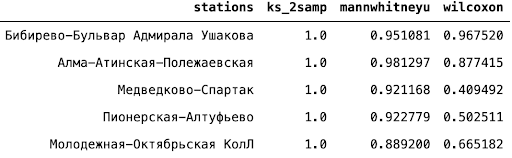
\includegraphics[scale=0.5]{pics/max_ks_2samp.png}
        \caption{Сравнение максимальных значений p-value критерия Колмогорова-Смирнова с результатами других критериев.}
        \label{max_ks_2samp}
    \end{figure}

    Теперь составим матрицу потоков на основе критерия однородности Колмогорова-Смирнова. Каждый элемент такой матрицы 
    содержит p-value для некоторой пары станций. На этом этапе мы отбирали станции, в которых были наиболее уверены, 
    был принят уровень значимости $\alpha = 1\%$. Кроме того, мы игнорировали пары с недостаточным количеством наблюдений, 
    то есть маршруты, которыми почти не пользовались.

    На основании этой матрицы мы выявили множества стоков и истоков, то есть станции, с которых люди не возвращаются (приезжает 
    больше, чем уезжает), и, наоборот, станции, куда люди не возвращаются (уезжает больше, чем приезжает). Для упрощения 
    анализа полученных данных была составлена карта стоков и истоков (Рис. \ref{large_flow}), однако пока она нуждается в доработке. 

    \begin{figure}[ht]
        \centering
        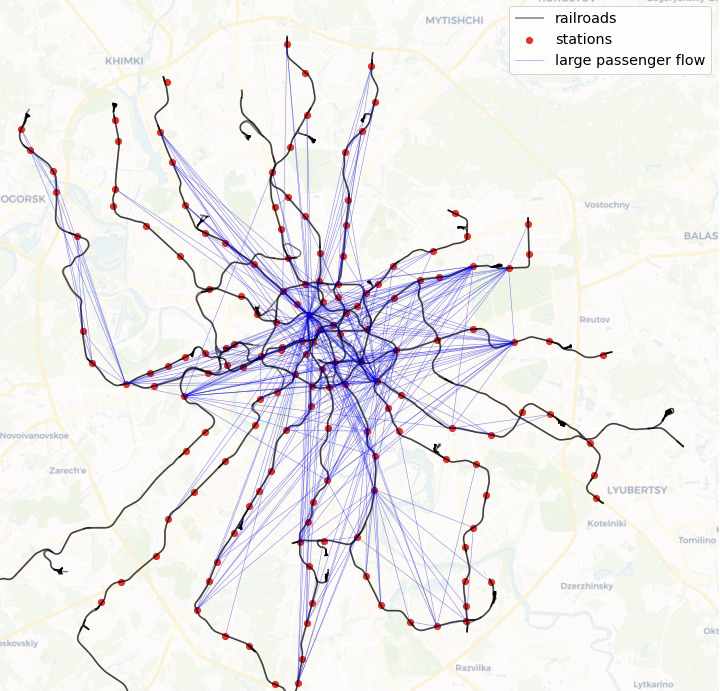
\includegraphics[scale=0.5]{pics/large_flow.png}
        \caption{Маршруты с наибольшим пассажиропотоком.}
        \label{large_flow}
    \end{figure}

    Поскольку даже отобранных пар станций оказалось слишком много (порядка восьми тысяч), для отображения на карте были выбраны только 
    самые "сильные" потоки, то есть потоки, в которых на одну станцию людей приезжает значительно больше, чем на другую (за весь рассматриваемый 
    период модуль разницы превышает \textbf{20000}). На карте не отображаются направления потоков, потому что они были бы едва ли различимы. 
    Отметим лишь, что в крупных скоплениях потоки зачастую имеют одинаковую направленность.

    Полученная информация о стоках и истоках является уникальной характеристикой транспортной системы, которая 
    отражает её текущее состояние и позволяет отслеживать намечающиеся тенденции. Например, станции Партизанская 
    и Шоссе Энтузиастов, которые являются стоками, фактически служат входом в Измайловский парк, точку притяжения 
    жителей Москвы. То же можно сказать и про Театральную~--- одну из самых загруженных станций города.

    \section{Оценка продолжительности поездки}

    Как уже упоминалось выше, мы работаем с агрегированными данными. 
    Это означает, что при обработке данных часть информации была утеряна, и теперь мы не 
    можем рассуждать в терминах единичных поездок. Нам доступны только получасовые интервалы 
    и агрегированные на них числовые показатели.

    Мы хотели бы получить распределения продолжительности поездки между различными парами станций. Задача восстановления плотности 
    распределения является классической для статистики и имеет много готовых решений. Однако все эти методы в нашем случае не работают, 
    потому что во время агрегации данных информация о продолжительности каждой конкретной поездки была утеряна. 

    Поэтому в этот раз классическая задача восстановления распределения имеет иную форму. На входе мы имеем количество человек, приезжающих 
    и уезжающих каждые полчаса, а на выходе должны получить распределение по времени. 
    Разобьём эту задачу на две части: первая заключается в получении выборки, состоящей из продолжительности некоторых поездок между 
    фиксированной парой станций, а вторая в построении вероятностного распределения на основе этой выборки. Для начала рассмотрим 
    пару вариантов решения первой части этой задачи.

    \subsection{Подготовка данных}

    Для проведения экспериментов снова обратимся к упрощённому случаю двух станций.
    Также, как и в прошлый раз, из общей совокупности поездок выберем только те, которые соединяют Университет и 
    Речной вокзал, при этом зафиксируем одно направление движения, пусть это будет путь от Университета до 
    Речного вокзала. Учтем условную смену дат метрополитена. 

    Только теперь мы не будем проводить укрупнение по дням, но на основании дат составим 28 отдельных таблиц следующего вида.

    \begin{center}
    \begin{tabular}{ |c|c|c| } 
        
        \hline
        получасовой интервал & число выехавших со & число прибывших на \\
        (только время) & станции отправления & станцию прибытия \\
        \hline
        \multicolumn{3}{c}{\footnotesize Таблица 4.
        Формат данных, агрегированных для вычисления времени поездки.} \\
        
    \end{tabular}
    \end{center}

    Каждая таблица содержит столбец получасовых интервалов, на которые разбивается весь рабочий день метрополитена, и два 
    столбца, характеризующих пассажирские потоки. Число выехавших и число прибывших обычно различаются, потому что зачастую 
    поездка от одной станции до другой занимает более чем полчаса. Эту особенность данных мы и используем для предсказания времени 
    поездки. Некоторые получасовые интервалы могут отсутствовать в таблице, это значит, что таких наблюдений не встречалось. 
    Добавим их, заполняя поля для количества пассажиров нулями.

    Во всех случаях мы вычисляем длину поездки для каждого конкретного дня.

    \subsection{Постановка задачи}

    Нам даны 28 таблиц вида (Таблица 4). Каждая такая таблица имеет 38 строчек, именно столько получасовых интервалов проходит за 
    время работы метрополитена ежедневно. Мы будем рассматривать столбцы 2 и 3 таблицы как отдельные выборки $x^i$ и $y^i$, соответствующие 
    пассажирам, вошедшим на одной станции, и пассажирам, вышедшим на другой. Таким образом, мы имеем 28 пар выборок $(x^i, y^i), i = 1, 2, \dots 28$, 
    где $x^i = (x^i_1, x^i_2, \dots, x^i_{38})$ и $y^i = (y^i_1, y^i_2, \dots, y^i_{38})$.

    Обозначим продолжительность поездки, которую мы хотим найти, как $D$. Вообще говоря, $D$ является случайной величиной, распределение 
    которой мы хотим получить по итогу решения задачи.

    На этом же этапе мы хотим предсказать условное математическое ожидание продолжительности поездки в каждый день месяца $\mathbb{E}_i D$, 
    где $i = 1, 2, \dots, 28$. Для этого были применены два метода, основанные на различных предположениях:
    
    \begin{itemize}
    \item \textbf{В первом методе} считается, что $D$~--- это дискретная величина, которая не обязана 
    совпадать для двух различных поездок. Алгоритм решения близок к умному перебору.
    
    \item \textbf{Второй же метод} предполагает, что в каждый отдельный день $D$ является вещественной константой.
    В этом случае задача сводится к условной выпуклой оптимизации.
    \end{itemize}

    \subsubsection{Первый способ}

    Этот метод основан на “окнах”. Изначально мы имеем по две выборки $x^i$ и $y^i$ из постановки задачи 
    для каждого дня месяца, представим их в виде упорядоченных по 
    временным интервалам массивов: выехавшие и прибывшие пассажиры. Сначала итерируемся по первому массиву 
    (выехавшие) и с его помощью пытаемся привести к нулю все элементы второго массива.
    
    Рассматривается некоторое “окно”~--- “правая” (увеличение индекса) окрестность элемента массива. 
    В нашем примере ширина окна равна $3$, что соответствует максимальному отступу “вправо” на $3$ элемента массива. 

    \begin{figure}[ht]
        \centering
        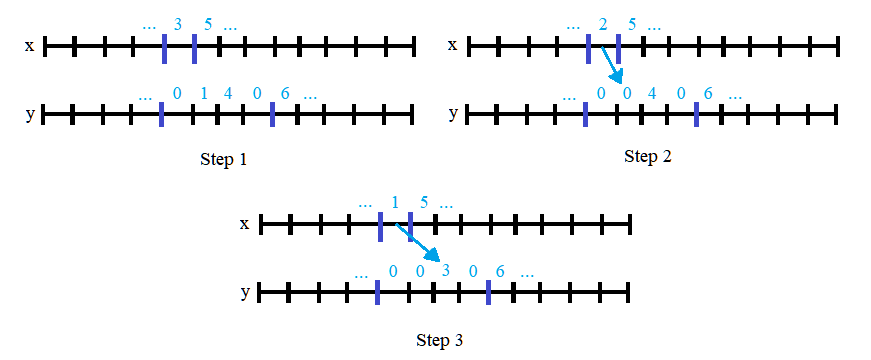
\includegraphics[scale=0.5]{pics/algo_time1.png}
        \caption{Пример работы первого способа предсказания времени поездки.}
        \label{algo_time1}
    \end{figure}
    
    Разберём обработку $i$-го элемента первого массива. В соответствие этому элементу поставим “окно” 
    во втором массиве с началом в $i$-ой позиции, то есть подмассив, занимающий элементы с $i$-го по $(i+1)$-й 
    включительно. Далее будем проводить следующий итеративный процесс: уменьшим $i$-ый элемент из первого 
    массива и ненулевой элемент из второго массива с минимальным номером из рассматриваемого “окна”. 
    В результате одной такой итерации получим значение отступа от начала “окна” (число от $0$ до $k$). 
    Этот итеративный процесс будет продолжаться до тех пор, пока либо $i$-ый элемент из первого массива 
    не обратится в $0$, либо в $0$ обратятся все элементы рассматриваемого “окна”.
    
    В итоге подобный процесс будет применен к каждому элементу первого массива. В результате его выполнения 
    мы будем получать различные значения отступа от начала “окна”. Для их подсчёта заведём массив $p$ длиной $(k+1)$, 
    $i$-ый элемент которого будет содержать количество отступов на $i$, совершенных во время выполнения алгоритма.
    Пример работы алгоритма приведён на Рис. \ref{algo_time1}.
    
    Если мы вспомним про природу данных, то поймём, что значение отступа характеризует продолжительность 
    поездки (кратную $30$ минутам). Для предсказания средней продолжительности поездки нам нужно усреднить полученные 
    результаты. Сложим все возможные продолжительности поездок, кратные $30$ минутам (в нашем случае это $30$, $60$, $90$ 
    и $120$ минут), умноженные на частоту их появления (то есть элементы нормированного массива $p$).
    
    Также мы можем полагать, что продолжительности поездок, соответствующие различным значениям отступа, равны $0$, 
    $30$, $60$ и $90$ минут соответственно. Это будет являться нижней оценкой продолжительности поездки, в то время как 
    изначальные вычисления выражают верхнюю оценку.

    В итоге получим, что $D \in [<lower, \hat{p}>, <upper, \hat{p}>]$, где $<.,.>$~--- скалярное произведение, $\hat{p}$~--- 
    нормированный вектор $p$, а upper и lower~--- векторы вида $(30, 60, 90, 120)$ и $(0, 30, 60, 90)$ соответственно.

    \subsubsection{Второй способ}

    В этом методе мы изначально предполагаем, что все поездки в один день одинаковы по продолжительности. 
    В таком случае можно считать, что упорядоченная выборка приезжающих пассажиров $x^i$ сдвинута относительно 
    упорядоченной выборки отъезжающих пассажиров $y^i$ на некоторое число. Это число и есть искомое математическое ожидание
    $D$. В этом случае в рамках одного дня справедливо равенство $D = \mathbb{E}_i D$. $x^i$ и $y^i$ имеют одинаковый 
    размер $n=38$.
    
    Чтобы найти искомый сдвиг выборки, перейдем к задаче оптимизации.

    $$
    \sum_{t=1}^{n - \lambda}L(x^i_t, y^i_{t + \lambda}) \rightarrow min_{\lambda}, 
    $$

    где $L$~--- функционал ошибки, а $\lambda$~--- дискретный сдвиг между выборками.

    В качестве функционала ошибки выберем квадрат разности $L(x, y) = (x - y)^2$. 
    Мы предполагаем, что поездка на метро не может длиться более двух часов. 
    Также в силу специфики задачи мы считаем $\lambda > 0$. В таком случае $\lambda$ принимает всего 
    $4$ значения и задачу можно решить перебором.

    $$
    \sum_{t=1}^{n - \lambda}(x^i_t - y^i_{t + \lambda})^2 \rightarrow min_{\lambda}
    $$

    В качестве ответа мы бы хотели получить число в диапазоне от $0$ до $120$~--- искомый сдвиг в
    минутах. Однако в представленных данных наше время дискретно, 
    то есть между $i$-ым и $(i+1)$-ым элементами выборки временная разница в $30$ минут. 
    Чтобы решить эту проблему и сдвигать одну выборку относительно другой на произвольное время, 
    применим метод линейного сглаживания относительно $y^i$. Тогда мы придем к следующей задаче оптимизации

    $$
        \sum_{t = 1}^{n - 1 - j}(x^i_t - (1 - \lambda_j) \ y^i_{t + j} - \lambda_j \ y^i_{t + 1 + j})^2 
        \rightarrow min_{\lambda_j} , \quad 0 \le \lambda_j \le 1, \quad j = 0, \dots, 3.
    $$

    Здесь мы применяем метод линейного сглаживания отдельно к каждому значению $\lambda$  
    для увеличения точности, $\lambda_j, j = 0, \dots, 3$ являются коэффициентами линейного сглаживания, 
    обратный переход от $\lambda_j, j = 0, \dots, 3$ к $\lambda$ будет показан позже. 
    После решения каждой из четырех подзадач мы подставим полученные 
    значения оптимума в эти подзадачи и выберем глобальный оптимум путём сравнения значений функционалов.
    
    Каждая из подзадач является задачей выпуклой оптимизации с дополнительными ограничениями  
    $0 \le \lambda_j \le 1$. Для их решения достаточно взять производную от функционала и приравняем её к нулю. 
    Мы оптимизируем параболу, ветви которой направлены вверх, следовательно, экстремум всего один и это минимум. 
    В итоге оптимум будет искаться по формуле

    $$
    \lambda_j = \frac{\sum_{t=1}^{n-1-j}(x^i_t - y^i_{t+j})(y^i_{t+1+j} - y^i_{t+j})}{\sum_{t=1}^{n-1-j}(y^i_{t+1+j} - y^i_{t+j})^2}, \quad j = 0, 1, 2, 3.
    $$

    Дополнительные ограничения легко учесть, исходя из специфики исходного функционала. 
    Поскольку мы оптимизируем параболу с ветвями, направленными вверх, при выходе $\lambda_j$ за пределы отрезка 
    $[0, 1]$ достаточно за оптимум принять ближайшую к $\lambda_j$ границу этого отрезка.
    
    Чтобы теперь получить значение $D$ из $\lambda_j$, нужно применить обратное преобразование 
    вида $D = \mathbb{E}_i D = 30j(1 - \lambda_j)+ 30(j + 1)\lambda_j = 30(j + \lambda_j)$, которое возвращает нас к изначальной постановке задачи.

    \subsection{Результаты эксперимента}

    Применяя первый метод и вычисляя медиану по всем дням месяца, я получил нижнюю и верхнюю оценки 
    продолжительности поездки, {\bf равные $46.4$ и $76.4$ минутам соответственно}.

    Используя же второй метод, я получил предсказание средней продолжительности поездки, {\bf равное $44.8$ минутам}.
    
    Полученные значения недостаточно сильно согласуются друг с другом. Я бы назвал второй метод более 
    точным, так как его предсказание соответствует современным коммерческим решениям в области (прогноз Яндекс.Метро~--- $42$ минуты).
    
    Теперь мы имеем две выборки размера $n=28$: выборка $x$ содержит математические ожидания $D$, вычисленные первым способом, а выборка 
    $y$~--- вторым. Считая, что $\mathbb{E}_i D$~-- это усреднённое значение времени поездки за $i$-ый день месяца, применим классические 
    методы восстановления плотности распределения. 

    Но для начала введём меру для оценки качества полученных распределений.

    \begin{Def}{}
        \textbf{Информационным критерием Акаике (AIC)} называется 
        критерий, применяющийся исключительно для выбора из нескольких статистических моделей.

        В общем случае \textbf{AIC}:
        $${\mathit {AIC}}=2k-2\ln(L),$$
        где $k$~--- число параметров в статистической модели, 
        $L$~--- максимизированное значение функции правдоподобия модели.
    \end{Def}

    \begin{figure}
        \centering
        \captionsetup{justification=centering}
        \begin{minipage}{.5\textwidth}
          \centering
          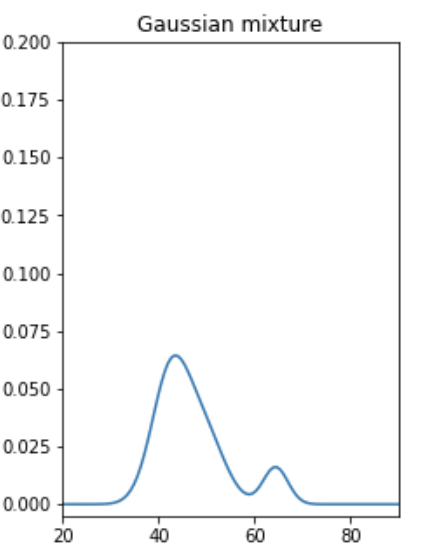
\includegraphics[width=.55\linewidth]{pics/dist_1.png}
          \captionof{figure}{Результат EM-алгоритма на \\данных первого метода.}
          \label{dist_1}
        \end{minipage}%
        \begin{minipage}{.5\textwidth}
          \centering
          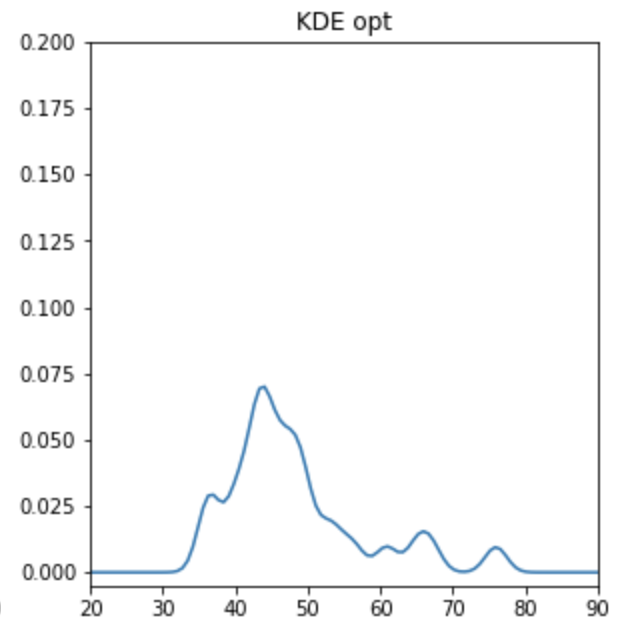
\includegraphics[width=.7\linewidth]{pics/dist_2.png}
          \captionof{figure}{Результат KDE на \\данных первого метода.}
          \label{dist_2}
        \end{minipage}
    \end{figure}

    Для построения распределений использовались два основных метода: EM-алгоритм для оценки смеси нормальных распределений и 
    ядерно сглаженная оценка плотности (Kernel density estimation, KDE). Поскольку KDE является непараметрическим алгоритмом 
    и для него не предусмотрена оценка сложности, он выступал в качестве сопровождающего метода. EM-алгоритм же поддаётся 
    оценке с помощью AIC, а потому был более предпочтителен.

    Нашей главной задачей является определение модальности полученного распределения. В случае смеси гауссиан число компонентов 
    смеси является гиперпараметром и характеризует модальность финального распределения. Поэтому наша задача сводится к подбору 
    оптимального значения этого параметра с целью минимизации информационного критерия AIC. 

    Для двух выборок $x$ и $y$ устроим перебор количества компонент смеси  $k$ в диапазоне $k \in [1, 5]$, такие границы 
    показались мне разумными, так как люди не склонны использовать очевидно неоптимальные маршруты при перемещении по городу 
    (количество же относительно оптимальных маршрутов обычно ограничивается тремя). 

    \begin{figure}
        \centering
        \captionsetup{justification=centering}
        \begin{minipage}{.5\textwidth}
          \centering
          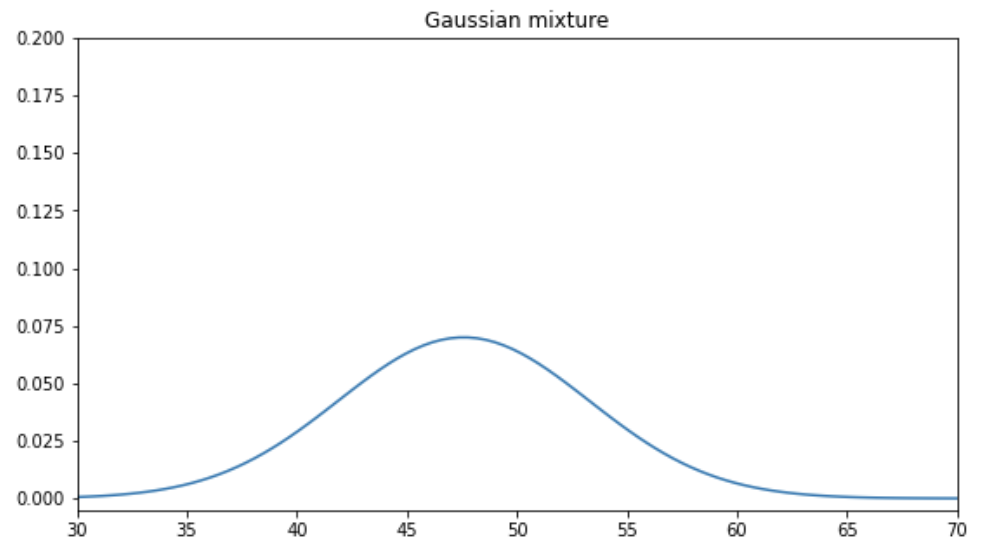
\includegraphics[width=\linewidth]{pics/dist_3.png}
          \captionof{figure}{Результат EM-алгоритма на \\данных второго метода.}
          \label{dist_3}
        \end{minipage}%
        \begin{minipage}{.5\textwidth}
          \centering
          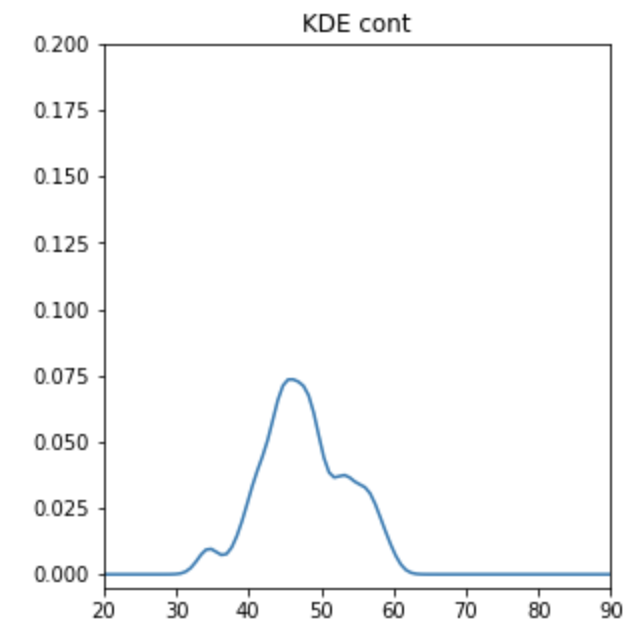
\includegraphics[width=.57\linewidth]{pics/dist_4.png}
          \captionof{figure}{Результат KDE на \\данных второго метода.}
          \label{dist_4}
        \end{minipage}
    \end{figure}

    Оптимальным значением для выборки $x$ оказалось $k=4$, AIC при этом равен $198$. Получившееся при этом распределение фактически 
    является бимодальным (Рис. \ref{dist_1}, \ref{dist_2}) и согласуется с KDE. Однако для выборки $y$ \quad $k=1$ (AIC = $181$) и результат EM-алгоритма 
    не согласуется с KDE, поэтому мы его отвергаем (Рис. \ref{dist_3}, \ref{dist_4}).

    Таким образом, мы считаем результирующее распределение бимодальным. Первый пик соответствует $D = 42$, что согласуется с уже полученными 
    результатами и подтверждается наблюдениями извне, второй же пик соответствует $D = 65$. То есть существует некоторый альтернативный маршрут, 
    который занимает явно больше времени, но популярен у значительной группы людей. Есть вероятность, что этот маршрут проходит через МЦК и 
    учитывает время, затраченное на пересадки, но этот факт требует дополнительного исследования.

    Кроме того, в рассмотренном методе всё ещё имеется несколько моментов, требующих прояснения. Например, почему результаты работы так 
    сильно зависят от способа получения математических ожиданий $D$, есть ли способ оценки сложности KDE и, наконец, как масштабировать этот 
    метод на всю транспортную сеть. Искать ответы на эти вопросы я планирую в дальнейших работах.

    \section{Заключение}

    На примере данных о пассажиропотоке московского метрополитена за февраль 2018 года были предложены два метода анализа 
    матрицы корреспонденций с целью изучения влияния внешних факторов на работу транспортной системы, эта задача уже 
    была поставлена, но до этого момента не имела решения. 
    
    Первый метод служит для 
    выявления точек интереса и транспортных узлов города, а второй метод позволяет изучать популярные маршруты в транспортной 
    системе и оценивать их эффективность с точки зрения затраченного времени. Оба подхода были реализованы с использованием 
    статистического аппарата и экспериментально проверены на предоставленных данных. В заключение стоит отметить, что 
    в обоих методах ещё есть простор для изучения и дальнейшей работы. 

    \newpage
    \bibliographystyle{plain}
    \addcontentsline{toc}{section}{Список литературы}
    \bibliography{reference}

\end{document}